%%%%%%%%%%%%%%%%%%%%%%%%%%%%%%%%%%%%%%%%%%%%%%%%%%%%%%%%%%%%%%%%%%%%%%%%
%                                                                      %
% This program is free software; you can redistribute it and/or modify %
% it under the terms of the GNU General Public License as published by %
% the Free Software Foundation; either version 2 of the License, or    %
% (at your option) any later version.                                  %
%                                                                      %
% This program is distributed in the hope that it will be useful,      %
% but WITHOUT ANY WARRANTY; without even the implied warranty of       %
% MERCHANTABILITY or FITNESS FOR A PARTICULAR PURPOSE.  See the        %
% GNU General Public License for more details.                         %
%                                                                      %
% You should have received a copy of the GNU General Public License    %
% along with this program; if not, write to the Free Software          %
% Foundation, Inc., 51 Franklin St, Fifth Floor, Boston,               %
% MA  02110-1301  USA                                                  %
%                                                                      %
%%%%%%%%%%%%%%%%%%%%%%%%%%%%%%%%%%%%%%%%%%%%%%%%%%%%%%%%%%%%%%%%%%%%%%%%
%
%	$Id$
%

\section{\label{ann-edt-vi}Commandes de base de l'{\'e}diteur {\tt vi}}

%%%%%%%%%%%%%%%%%%%%%%%%%%
\subsection{\label{ann-edt-vi-intro}Introduction et conventions}

Cette section donne un aper\c{c}u du fonctionnement de l'{\'e}diteur de
texte \index{vi@\texttt{vi}}"{\tt vi}". Cet {\'e}diteur est en standart sur l'ensemble des
syst{\`e}mes sous {\Unix}, voire m{\^e}me sur d'autres syst{\`e}mes
d'exploitation comme {\OpenVMS}, {\DOS}, {\MacOS}, {\Windows} et
{\WindowsNT}. Par cons{\'e}quent, {\`a} partir d'une installation de
base de quelqu'{\Unix} que ce soit, vous aurez toujours "{\tt vi}"
{\`a} votre disposition. De m{\^e}me, c'est cet {\'e}diteur qui est
utilis{\'e} par d{\'e}faut pour de nombreuses commandes de configuration
du syst{\`e}me, car, peut importe le type de terminal utilis{\'e} pour
la console d'administration, "{\tt vi}" vous permettra d'{\'e}diter
les diff{\'e}rents fichiers de configuration.

"{\tt vi}" souffre d'une tr{\`e}s mauvaise image de par son peu de
convivialit{\'e}. Cependant, il peut {\^e}tre utilis{\'e} sur n'importe
quel type de terminal {\ASCII}, contrairement {\`a} {\tt LSEDIT} sur
{\OpenVMS} et dispose de nombreuses fonctionnalit{\'e}s facilitant
l'{\'e}criture de programmes complexes.

Par contre, contrairement {\`a} <<{\tt emacs}", "{\tt vi}" n'est
pas un {\'e}diteur programmable, c'est-{\`a}-dire extensible gr{\^a}ce
{\`a} un langage de programmation.

Dans toute la suite, les conventions suivantes seront utilis{\'e}es~:
\begin{itemize}
	\item	Toute commande pr{\'e}c{\'e}d{\'e}e par le caract{\`e}re
			"{\tt :}" correspond {\`a} une commande interne {\`a}
			"{\tt vi}". Par cons{\'e}quent, elle doit {\^e}tre valid{\'e}e
			par {\returnkey}.
	\item	{\sl fichier} d{\'e}signe le nom d'un fichier.
	\item	{\sl cmd\_curseur} d{\'e}signe une commande li{\'e}e au
			d{\'e}placement du curseur dans "{\tt vi}".
	\item	{\sl caract} d{\'e}signe un et un seul caract{\`e}re.
	\item	{\sl str} d{\'e}signe une cha{\^\i}ne de caract{\`e}res ou bien
			une expression r{\'e}guli{\`e}re (cf. chapitre \ref{reg-exp}).
	\item	{\sl n,m} repr{\'e}sentent~:
		\begin{itemize}
			\item[$\star$]  soit deux num{\'e}ros de lignes,
					par exemple "\verb=4,50=",
			\item[$\star$]	soit deux marqueurs de lignes,
					par exemple "\verb=.,$=",
			\item[$\star$]	soit deux expressions de recherche utilisant
					les expressions r{\'e}guli{\`e}res (cf. chapitre \ref{reg-exp}),
					par exemple "\verb*=/recherche 1/,/recherche 2/=",
			\item[$\star$]	soit toute combinaison possible des trois
					possibilit{\'e}s pr{\'e}c{\'e}dentes, par exemple "\verb=1,.=",
					"\verb*=/recherche 1/,$=".
		\end{itemize}
	\item	{\sl (a-z)} d{\'e}signe n'importe quel caract{\`e}re de "{\tt a}" {\`a}
			"{\tt z}"
\end{itemize}

Nous avons introduit la notion de marqueur de ligne. Un marqueur est une
convention pour d{\'e}signer certaines lignes particuli{\`e}res dont il n'est pas
possible de d{\'e}terminer le num{\'e}ro {\`a} l'avance. Les deux marqueurs pr{\'e}d{\'e}finis
dans "{\tt vi}" sont~:

\begin{longtable}{|l|p{10cm}|}
	\multicolumn{2}{r}{{\sl Suite page suivante $\cdots$}}	\\
\endfoot
\endlastfoot
	\hline
		\multicolumn{1}{|c|}{Marqueur}				&
		\multicolumn{1}{|c|}{Description}			\\
	\hline \hline
		{\tt .}		&	ligne courante, c'est-{\`a}-dire la ligne o{\`u} se trouve
						actuellement le curseur,	\\
	\hline
		\verb=$=	&	fin de fichier				\\
	\hline
\end{longtable}

%%%%%%%%%%%%%%%%%%%%%%%%%%
\subsection{\label{ann-edt-vi-fcts}Modes de fonctionnement de "{\tt vi}"}

"{\tt vi}" distingue deux modes de fonctionnements~:
\begin{description}
	\item[{\rm le mode "{\sl commande}"}]\mbox{}\\
		Ce mode correspond lorsque vous n'{\^e}tes pas en train de saisir du texte.
		Pour cela, chaque touche du clavier alphanum{\'e}rique correspond {\`a} une
		fonctionnalit{\'e} de l'{\'e}diteur de texte. Vous pouvez d{\'e}placer le curseur,
		recher\-cher du texte, sauvegarder le {\sl buffer} courrant, appeler le
		{\sl prompt} de "{\tt vi}" afin de saisir des commandes
		internes de l'{\'e}diteur. Comme tout utilitaire {\Unix},
		"{\tt vi}" fait la diff{\'e}rence entre les majuscules et les minuscules.
		Par cons{\'e}quent, {\bf vous devez prendre garde que la touche \key{{\sc Caps}}
		ou "{\sl Verrouillage en majuscule}" ne soit pas en fonction}. Dans
		ce cas, le comportement que pourrait avoir "{\tt vi}" risque de
		vous surprendre et {\bf surtout} ne pas faire ce que vous souhait{\'e} (mais
		par contre ce qui a {\'e}t{\'e} demand{\'e} !).\\[2ex]
	\item[{\rm le mode "{\sl insertion}"}]\mbox{}\\
		Ce mode correspond lorsque vous {\^e}tes en train de saisir ou de modifier
		du texte. Vous pouvez ins{\'e}rer autant de lignes que vous voulez, par contre,
		vous ne pouvez modifier le texte que de la ligne courrant.
		
		Pour quitter le mode "{\sl insertion}", il vous suffit d'appuyer
		sur la touche {\esckey}.
\end{description}

{\`A} la section \ref{ann-edt-vi-intro}, nous avons parl{\'e} de commandes
"{\tt vi}" commen\c{c}ant par le caract{\`e}re "{\tt :}" et valid{\'e}e par
{\returnkey}. Ce mode de fonctionnement correspond au "{\sl prompt}"
de "{\tt vi}", invite {\`a} partir de laquelle il est possible de saisir
des commandes internes {\`a} "{\tt vi}". Ce mode est accessible {\`a} partir
du mode "{\sl commande}". Les diff{\'e}rences entre ces deux comportements
sont les suivantes~:
\begin{itemize}
	\item	En mode {\sl commande}, toutes les touches du clavier
			alphanum{\'e}rique ont une fonction particuli{\`e}re, par exemple
			pour d{\'e}placer le curseur, effacer des caract{\`e}res ou des lignes,
			s{\'e}lectionner du texte, etc. Ce mode serait l'{\'e}quivalent, sous
			les {\'e}diteurs de texte de {\OpenVMS}, d'acc{\'e}der {\`a} toutes les
			fonction\-nalit{\'e}s des touches du pav{\'e} num{\'e}rique sur des claviers
			LK200, LK400. En effet, pour ces {\'e}diteurs, chaque touche
			correspond {\`a} une fonctionnalit{\'e} donn{\'e}e. Sous "{\tt vi}",
			le clavier num{\'e}rique est cens{\'e} permettre d'afficher des nombres
			ou d'utiliser les fl{\`e}ches (sur des claviers de type PC). Il a
			donc fallu trouver une m{\'e}thode pour associer des raccourcis
			clavier {\`a} un certain nombre de fonctionnalit{\'e}. L'une d'entre
			elle est d'acc{\'e}der au "{\sl prompt}" de "{\tt vi}"
			afin de saisir des commandes internes {\`a} l'{\'e}diteur.\\[2ex]
	\item	{\`A} l'invite de "{\tt vi}", il est possible de saisir
			un certain nombre de commandes explicit{\'e}es dans toute la suite.
			Ces commandes servent {\`a} d{\'e}finir l'environ\-nement de travail,
			ex{\'e}cuter des actions, etc. Pour y acc{\'e}der, il suffit d'appuyer
			sur la touche \key{:} {\`a} partir du mode commande. Ce mode de
			fonctionnement est {\'e}quivalent {\`a} celui des {\'e}diteurs de texte
			sous {\OpenVMS} une fois que la touche \key{{\sc do}} est
			press{\'e}e.
\end{itemize}

Dans tout ce qui suit, les commandes explicit{\'e}es sont valables en
mode "{\sl commande}" {\`a} moins que celui-ci ne soit pr{\'e}cis{\'e}. Toutes
les commandes pr{\'e}c{\'e}d{\'e}es par le caract{\`e}re <<{\tt :}" sont accessibles
{\`a} partir du "{\sl prompt}" de "{\tt vi}". Pour appeler le
prompt, il suffit de~:
\begin{enumerate}
	\item	{\^e}tre en mode "{\sl commande}",
	\item	appuyer sur la touche \key{:}.
\end{enumerate}

%%%%%%%%%%%%%%%%%%%%%%%%%%
\subsection{\label{ann-edt-vi-start}D{\'e}marrage d'une session "{\tt vi}"}

\begin{longtable}{p{4cm}@{\hspace{0.5cm}}p{7cm}}
	\multicolumn{2}{r}{{\sl Suite page suivante $\cdots$}}	\\
\endfoot
\endlastfoot
	{\tt vi} {\sl fichier}	&
		{\'E}dite {\sl fichier}.	\\[2ex]
	{\tt vi -r } {\sl fichier}	&
		{\'E}dite la derni{\`e}re version sauvegard{\'e}e de {\sl fichier}
		apr{\`e}s une sortie anormale de l'{\'e}diteur de texte. Cette
		option est l'{\'e}quivalent de la commande "{\tt RECOVER BUFFER}"
		sous l'{\'e}diteur "{\tt LSEDIT}" sous {\OpenVMS}.	\\[2ex]
	{\tt vi +}{\sl n fichier}	&
		{\'E}dite {\sl fichier}	et place le curseur directement {\`a} la ligne
		{\sl n}.\\[2ex]
	{\tt vi +} {\sl fichier}	&
		{\'E}dite {\sl fichier}	et place le curseur directement sur
		la derni{\`e}re ligne.\\[2ex]
	{\tt vi} {\sl fichier1 fichier2 $\cdots$ fichiern}	&
		{\'E}dite successivement les fichiers {\sl fichier1 fichier2
		$\cdots$ fichiern}. Le passage ne peut se faire que du pr{\'e}c{\'e}dent
		au suivant (donc pas de remont{\'e}e possible). La commande
		pour passer au fichier suivant est "{\tt :n}". Si le fichier
		n'a pas {\'e}t{\'e} sauvegard{\'e}, un message d'alarme est affich{\'e} et le
		passage au fichier suivant n'est pas effectu{\'e}. Si, toute fois
		vous d{\'e}sirez forcer ce passage, tapez la commande "\verb=:n!=".
		\\[2ex]
	{\tt vi +/}{\sl str fichier}	&
		{\'E}dite {\sl fichier}	et place le curseur directement sur
		la premi{\`e}re ligne contenant la cha{\^\i}ne "{\sl str}".\\[2ex]
\end{longtable}

%%%%%%%%%%%%%%%%%%%%%%%%%%
\subsection{\label{ann-edt-vi-quit}Sauvegarder et quitter "{\tt vi}"}

\begin{longtable}{p{4cm}@{\hspace{0.5cm}}p{7cm}}
	\multicolumn{2}{r}{{\sl Suite page suivante $\cdots$}}	\\
\endfoot
\endlastfoot
	\verb=ZZ= ou \verb=:wq= ou \verb=:x=
		&	Sortie avec sauvegarde.	\\[2ex]
	\verb*=:w ={\sl fichier}
		&	Sauvegarde le contenu de l'{\'e}diteur dans le fichier
			nomm{\'e} "{\sl fichier}". Si aucun nom n'est donn{\'e},
			celui pris en compte sera celui du fichier courrant.
			\\[2ex]
	{\tt :w!}~{\sl fichier}
		&	Force la sauvegarde du fichier. Si aucun nom n'est donn{\'e},
			celui pris en compte sera celui du fichier courrant.
			\\[2ex]
	{\tt :}{\sl n}{\tt ,}{\sl m}\verb*=w ={\sl fichier}
		&	Sauvegarde de la ligne "{\sl n}" {\`a} la ligne
			"{\sl m}" dans le fichier
			nomm{\'e} "{\sl fichier}". Si aucun nom n'est donn{\'e},
			celui pris en compte sera celui du fichier courrant.
			\\[2ex]
	{\tt :}{\sl n}{\tt ,}{\sl m}\verb*=w>>={\sl fichier}
		&	Sauvegarde de la ligne "{\sl n}" {\`a} la ligne
			"{\sl m}"{\`a} la fin du fichier
			nomm{\'e} "{\sl fichier}". Si aucun nom n'est donn{\'e},
			celui pris en compte sera celui du fichier courrant.
			\\[2ex]
	{\tt :q}
		&	Quitte "{\tt vi}" sans sauvegarde. Si toutefois des
			modifications ont {\'e}t{\'e} effectu{\'e}es, "{\tt vi}" le signalera
			et annulera l'op{\'e}ration de sortie.
			\\[2ex]
	{\tt :q!}
		&	Force la sortie de "{\tt vi}" sans sauvegarde. Si des
			modifications ont {\'e}t{\'e} effectu{\'e}es, aucun message ne
			sera affich{\'e} et les modifications seront perdues.
			\\[2ex]
	{\tt :e!}
		&	Permet d'annuler toutes les modifications effectu{\'e}es depuis
			la derni{\`e}re sauvegarde.
			\\[2ex]
\end{longtable}

{\Large \bf \sc Attention}~:
\begin{quote}
Aucune sauvegarde de la version pr{\'e}c{\'e}dente n'est effectu{\'e}e. Si vous
sortez de "{\tt vi}" avec sauvegarde ou bien si vous sauvegardez
les modifications faites, aucune trace de votre pr{\'e}c{\'e}dent travail
ne sera conserv{\'e}e.
\end{quote}

%%%%%%%%%%%%%%%%%%%%%%%%%%
\subsection{\label{ann-edt-vi-stat}Commandes d'{\'e}tat}

\begin{longtable}{p{4cm}@{\hspace{0.5cm}}p{7cm}}
	\multicolumn{2}{r}{{\sl Suite page suivante $\cdots$}}	\\
\endfoot
\endlastfoot
	\verb,:.=,	&	Affiche le num{\'e}ro de la ligne courrante.	\\[2ex]
	\verb,:=,	&	Affiche le nombre de lignes du fichier charg{\'e} dans
					l'{\'e}diteur.\\[2ex]
	\control{g}	&	Affiche le nom du fichier trait{\'e}, le num{\'e}ro de la
					ligne courrante,le nombre total de lignes et le
					pourcentage relatif de la position courrante.\\[2ex]
\end{longtable}


%%%%%%%%%%%%%%%%%%%%%%%%%%
\subsection{\label{ann-edt-vi-insert}Insertion de texte}

\begin{longtable}{p{4cm}@{\hspace{0.5cm}}p{7cm}}
	\multicolumn{2}{r}{{\sl Suite page suivante $\cdots$}}	\\
\endfoot
\endlastfoot
	{\tt a}		&	Ajoute du texte {\bf apr{\`e}s} la position courrante du
					curseur.\\[2ex]
	{\tt A}		&	Ajoute du texte apr{\`e}s la fin de la ligne
					courrante.\\[2ex]
	{\tt i}		&	Ins{\`e}re du texte {\bf avant} la position courrante du
					curseur.\\[2ex]
	{\tt I}		&	Ins{\`e}re du texte au d{\'e}but de la ligne courrante.\\[2ex]
	{\tt o}		&	Ouvre une nouvelle ligne {\bf en dessous} de la
					ligne courrante.\\[2ex]
	{\tt O}		&	Ouvre une nouvelle ligne {\bf au dessus} de la ligne courrante.\\[2ex]
	\control{v}{\sl caract}	&	
					En mode insertion, cette commande permet d'ins{\'e}rer
					n'importe quel caract{\`e}re de controle, comme {\esckey},
					un saut de page, etc. Par exemple, pour ins{\'e}rer
					le caract{\`e}re {\esckey} dans le fichier, il suffit
					de taper la s{\'e}quence suivante {\bf en mode insertion}~:
					\\
				&	\multicolumn{1}{c}{\control{v}~~{\esckey}}	\\[2ex]
	\verb*=:r ={\sl fichier}	&
					Lit le fichier pass{\'e} en argument et l'ins{\`e}re apr{\`e}s
					la ligne courrante.\\[2ex]
	{\tt :}{\sl n}\verb*=r ={\sl fichier}	&
					Lit le fichier pass{\'e} en argument et l'ins{\`e}re apr{\`e}s
					la ligne "{\sl n}".
\end{longtable}

La figure \ref{ann-edt-vi-insert-fig} r{\'e}sume les commandes
pr{\'e}c{\'e}dentes.

\begin{figure}[hbtp]
%\epsfbox{_Images/ann-edt-vi/insert-cmds.eps}
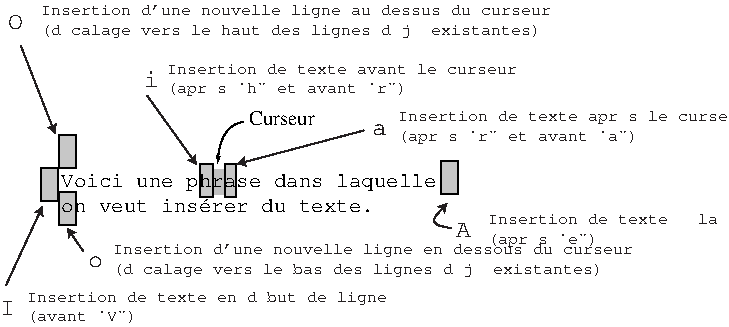
\includegraphics{ann-edt-vi/insert-cmds}
\caption{\label{ann-edt-vi-insert-fig}R{\'e}sum{\'e} des commandes d'insertion
	de texte de "{\tt vi}".}
\end{figure}

\begin{remarque}
Toutes les commandes d'insertion pr{\'e}sent{\'e}es ici, permettent
d'ins{\'e}rer plusieurs lignes. En effet, il suffit de taper son texte
{\it au kilom{\`e}tre} et presser sur la touche {\returnkey} pour
cr{\'e}er une autre ligne, comme tout autre {\'e}diteur de texte
{\it pleine page}. Par contre, vous ne pouvez revenir en arri{\`e}re que sur
la m{\^e}me ligne que le curseur. Si vous d{\'e}sirez revenir sur une
ligne pr{\'e}c{\'e}dente, que vous avez saisi sans sortir du mode
insertion, {\bf il vous faudra revenir en mode commande pour vous y
placer}.
\end{remarque}


%%%%%%%%%%%%%%%%%%%%%%%%%%
\subsection{\label{ann-edt-vi-undo}Annuler ou r{\'e}p{\'e}ter des commandes}

\begin{longtable}{p{4cm}@{\hspace{0.5cm}}p{7cm}}
	\multicolumn{2}{r}{{\sl Suite page suivante $\cdots$}}	\\
\endfoot
\endlastfoot
	{\tt u}		&
		Annule la derni{\`e}re commande.
		\\[2ex]
	{\tt U}		&
		Restaure la ligne courrante {\`a} son {\'e}tat d'origine.
		\\[2ex]
%%	{\tt "}{\sl n}{\tt p}	&
%%		A VOIR
%%		\\[2ex]
%%	{\tt "1pu.uu}	&
%%		A VOIR
%%		\\[2ex]
	{\tt n}		&
		R{\'e}p{\`e}te la derni{\`e}re op{\'e}ration de recherche "{\tt /}" ou "{\tt ?}".
		(cf. section \ref{ann-edt-vi-search}). Cette op{\'e}ration s'effectue de la
		position courrante vers la fin du fichier.
		\\[2ex]
	{\tt N}		&
		R{\'e}p{\`e}te la derni{\`e}re op{\'e}ration de recherche "{\tt /}" ou "{\tt ?}".
		(cf. section \ref{ann-edt-vi-search}). Cette op{\'e}ration s'effectue {\bf
		en sens inverse}, c'est-{\`a}-dire de la position courrante vers {\bf le
		d{\'e}but du fichier}.
		\\[2ex]
	{\tt ;}		&
		R{\'e}p{\`e}te la derni{\`e}re commande de recherche "{\tt f}", "{\tt F}",
		"{\tt t}" ou "{\tt T}" (cf. section \ref{ann-edt-vi-searchop}).
		\\[2ex]
	{\tt ,}		&
		R{\'e}p{\`e}te la derni{\`e}re commande de recherche "{\tt f}", "{\tt F}",
		"{\tt t}" ou "{\tt T}" {\bf en sens inverse}(cf. section
		\ref{ann-edt-vi-searchop}).
		\\[2ex]
	{\tt .}		&
		R{\'e}p{\`e}te la derni{\`e}re op{\'e}ration de insertion/suppression ou modification
		de texte dans le fichier.
		\\[2ex]
\end{longtable}


%%%%%%%%%%%%%%%%%%%%%%%%%%
\subsection{\label{ann-edt-vi-move}D{\'e}placement du curseur}

\begin{longtable}{p{3cm}@{\hspace{0.5cm}}p{8cm}}
	\multicolumn{2}{r}{{\sl Suite page suivante $\cdots$}}	\\
\endfoot
\endlastfoot
	{\tt k} ou \control{p}					&
		D{\'e}placement vers le haut.		\\
	ou \key{$\uparrow$}						&
		\\[2ex]
	{\tt j} ou \control{j} 					&
		D{\'e}placement vers le bas.		\\
	ou \control{n} ou \key{$\downarrow$}	&
		\\[2ex]
	{\tt h} ou \control{h}					&
		D{\'e}placement vers la gauche			\\
	ou \key{{\small \sc Back Space}} ou \key{$\leftarrow$}	&
		\\[2ex]
	{\tt l} ou {\spacekey} ou \key{$\rightarrow$}	&
		D{\'e}placement vers la droite.
		\\[2ex]
	{\tt w} ou {\tt W}	&
		D{\'e}place le curseur au d{\'e}but du mot suivant. "{\tt W}" permet d'ignorer la
		ponctuation.
		\\[2ex]
	{\tt b} ou {\tt B}	&
		D{\'e}place le curseur au d{\'e}but du mot pr{\'e}c{\'e}dent. "{\tt B}" permet d'ignorer la
		ponctuation.
		\\[2ex]
	{\tt e} ou {\tt E}	&
		D{\'e}place le curseur {\`a} la fin du mot courrant. "{\tt E}" permet d'ignorer la
		ponctuation.
		\\[2ex]
	{\tt 0} (z{\'e}ro) ou {\tt |} (pipe)	&
		D{\'e}place le curseur {\`a} la premi{\`e}re colonne de la ligne courrante.
		\\[2ex]
	{\sl n}{\tt |} (pipe)	&
		D{\'e}place le curseur {\`a} la colonne "{\sl n}" de la ligne courrante.
		\\[2ex]
	\verb=^=	&
		D{\'e}place le curseur sur le premier caract{\`e}re diff{\'e}rent de l'espace ou de
		la tabulation sur la ligne courrante.
		\\[2ex]
	\verb=$=	&
		D{\'e}place le curseur {\`a} la fin de la ligne courrante.
		\\[2ex]
	{\tt +} ou {\returnkey}	&
		Deplace le curseur au d{\'e}but de la ligne suivante.
		\\[2ex]
	{\tt -}	&
		D{\'e}place le curseur sur le premier caract{\`e}re diff{\'e}rent de l'espace ou de la
		tabulation de la ligne pr{\'e}c{\'e}dente.
		\\[2ex]
	{\tt 1G}	&
		Ram{\`e}ne le cuseur {\`a} la premi{\`e}re ligne.
		\\[2ex]
	{\tt G}	&
		D{\'e}place le curseur {\`a} la fin du fichier.
		\\[2ex]
	\verb=G$=	&
		D{\'e}place le curseur {\`a} la fin de la derni{\`e}re ligne du fichier.
		\\[2ex]
	{\sl n}{\tt G}	&
		D{\'e}place le curseur {\`a} la $n^e$ ligne du fichier.
		\\[2ex]
	{\tt (}	&
		Ram{\`e}ne le curseur au d{\'e}but de la phrase courrante. Une phrase, pour "{\tt vi}"
		est une suite de mots s{\'e}par{\'e}s par des espaces ou des caract{\`e}res de ponctuations
		et termin{\'e}s par le caract{\`e}re "{\tt .}".
		\\[2ex]
	{\tt )}	&
		D{\'e}place le curseur au d{\'e}but de la phrase suivante.
		\\[2ex]
	\verb={=	&
		Ram{\`e}ne le curseur au d{\'e}but du paragraphe courrant. Un paragraphe, pour
		"{\tt vi}", est une suite de phrases s{\'e}par{\'e}s par une ligne blanche. Cette
		terminologie ob{\'e}it {\`a} la syntaxe de {\TeX} et de {\LaTeX}.
		\\[2ex]
	\verb=}=	&
		D{\'e}place le curseur au d{\'e}but du paragraphe pr{\'e}c{\'e}dent.
		\\[2ex]
\end{longtable}

La figure \ref{ann-edt-vi-movefig} d{\'e}crit les diff{\'e}rentes actions de ces commandes
en fonction de la position du curseur dans le fichier.

\begin{figure}[hbtp]
%\epsfbox{_Images/ann-edt-vi/move-cmds.eps}
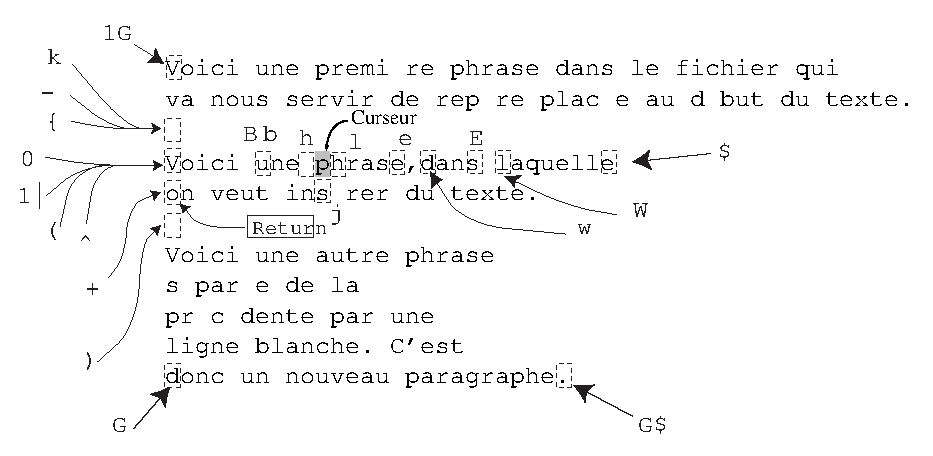
\includegraphics{ann-edt-vi/move-cmds}
\caption{\label{ann-edt-vi-movefig}Commandes de d{\'e}placement du curseur avec
"{\tt vi}".}
\end{figure}

Sachant que "{\tt vi}" a {\'e}t{\'e} d{\'e}di{\'e} aux d{\'e}veloppeurs {\Unix}, il est
clair que "{\tt vi}" reprend des notions du langage C. Lorsque la
premi{\`e}re colonne d'une ligne du fichier contient le caract{\`e}re
"\verb={=", "{\tt vi}" consid{\`e}re tout le texte compris entre ces
deux marques (texte compris entre deux "\verb={=" situ{\'e}s en premi{\`e}re
colonne) comme une section. Par exemple~:\\[2ex]
\begin{quote}
\begin{verbatim}
{
    Le caractere sur la ligne precedente permet de marquer une section.
    La prochaine section commencera des que le caractere { apparaitra
    a nouveau en premiere colonne dans le fichier.
{
    Ici nous sommes dans une nouvelle section. On pourrait faire l'analogie
    avec le langage C lorsque l'on declare le corps d'une
    fonction. En effet on aura :
main()
{
    section associee au corps de la fonction main.
    Donc nous sommes ici dans la troisieme section de ce fichier texte.
}

ma_fonction()
{
    section associee au corps de la fonction ma_fonction.
    Donc nous sommes ici dans la quatrieme section de ce fichier texte.
}
\end{verbatim}
\end{quote}

Pour se d{\'e}placer d'une section {\`a} l'autre, "{\tt vi}" dispose des commandes
suivantes~:

\begin{longtable}{p{4cm}@{\hspace{0.5cm}}p{7cm}}
	\multicolumn{2}{r}{{\sl Suite page suivante $\cdots$}}	\\
\endfoot
\endlastfoot
	\verb=[[=	&
		Ram{\`e}ne le curseur au d{\'e}but de la section courrante.
		\\[2ex]
	\verb=]]=	&
		D{\'e}place le curseur au d{\'e}but de la section suivante.
		\\[2ex]
\end{longtable}


%%%%%%%%%%%%%%%%%%%%%%%%%%
\subsection{\label{ann-edt-vi-del}Effacement de texte}

Dans toute la suite de cette section, le caract{\`e}re courrant d{\'e}signera
celui sur lequel est positionn{\'e} le curseur. De m{\^e}me, la ligne courrant
sera celle ou se trouve le curseur.

Pour "{\tt vi}", un mot est une s{\'e}quence de caract{\`e}res alphanum{\'e}riques
s{\'e}par{\'e}s par un ou plusieurs espaces ou tabulation ou bien encore un
caract{\`e}re de ponctuation. Le mot courrant d{\'e}signe la chaine de caract{\`e}re
{\bf commen\c{c}ant {\`a} la position du curseur} jusqu'{\`a} un caract{\`e}re valide de 
d{\'e}limitatio pour un mot.

\begin{longtable}{p{4cm}@{\hspace{0.5cm}}p{7cm}}
	\multicolumn{2}{r}{{\sl Suite page suivante $\cdots$}}	\\
\endfoot
\endlastfoot
	\control{h} ou \key{{\small \sc Back Space}}	&
		{\bf En mode insertion}, efface le caract{\`e}re pr{\'e}c{\'e}dent.
		\\[2ex]
	\control{w}	&
		{\bf En mode insertion}, efface le mot pr{\'e}c{\'e}dent.
		\\[2ex]
	\control{x}	&
		{\bf En mode \sl insertion}, efface tout le texte ins{\'e}r{\'e} depuis le d{\'e}but
		du mode "{\sl insertion}".
		\\[2ex]
	{\sl n}{\tt x}	&
		Efface les "{\sl n}" caract{\`e}res suivants y compris le caract{\`e}re
		courrant. Si "{\sl n}" n'est pas sp{\'e}cifi{\'e}, "{\tt vi}" n'efface
		que le caract{\`e}re courrant.
		\\[2ex]
	{\sl n}{\tt X}	&
		Efface les "{\sl n}" caract{\`e}res pr{\'e}c{\'e}dents y compris le caract{\`e}re
		courrant. Si "{\sl n}" n'est pas sp{\'e}cifi{\'e}, "{\tt vi}" n'efface
		que le caract{\`e}re pr{\'e}c{\'e}dent.
		\\[2ex]
	{\tt xp}	&
		Intervertit le caract{\`e}re courrant avec le caract{\`e}re suivant.
		\\[2ex]
	{\sl n}{\tt dw}	&
		Efface les "{\sl n}" mots suivants. Si "{\sl n}" n'est pas
		sp{\'e}cifi{\'e}, "{\tt vi}~�> d{\'e}truit le mot courrant. Pour rappel, un
		mot est une suite de caract{\`e}res s{\'e}par{\'e}s par un ou plusieurs espaces
		ou tabulation ou bien par un caract{\`e}re de ponctuation.
		\\[2ex]
	{\sl n}{\tt db}	&
		Efface les "{\sl n}" mots pr{\'e}c{\'e}dents. Si "{\sl n}" n'est pas
		sp{\'e}cifi{\'e}, "{\tt vi}~�> d{\'e}truit le mot courrant.
		\\[2ex]
	{\sl n}{\tt dd}	&
		Efface les "{\sl n}" lignes suivantes en commen\c{c}ant par la
		ligne courrante. Si <<n {\sl n}" n'est pas sp{\'e}cifi{\'e}, "{\tt vi}"
		ne d{\'e}truit que la ligne courrante.
		\\[2ex]
	{\tt :}{\sl n,m}{\tt d}	&
		D{\'e}truit les lignes de "{\sl n}" {\`a} "{\sl m}". Si 
		"$n \in \mathcal{N}$" ou "$m \in \mathcal{N}$", alors
		l'op{\'e}ration de destruction commence ou se termine {\`a} la ligne dont
		le num{\'e}ro est sp{\'e}cifi{\'e}. Si "{\sl n}" ou "{\sl m}" est un
		marqueur, l'op{\'e}ration de destruction commence ou se termine
		{\`a} la position indiqu{\'e}e par le marqueur (cf. section
		\ref{ann-edt-vi-intro}). Si "{\sl n}" ou "{\sl m}" est une
		expression r{\'e}guli{\`e}re d{\'e}limit{\'e}e par le caract{\`e}re "{\tt /}",
		l'op{\'e}ration commence {\`a} la premi{\`e}re ligne trouv{\'e}e {\`a} partir
		de la position courrant satisfaisant
		l'expression r{\'e}guli{\`e}re ou bien se termine {\`a} la {\bf premi{\`e}re}
		ligne  satisfaisant l'expression r{\'e}guli{\`e}re se trouvant
		{\`a} la suite de la premi{\`e}re ligne {\`a} effacer. 
		\\[2ex]
	{\tt D}	ou \verb=d$=	&
		D{\'e}truit tout ce qui suit {\`a} partir de la position courrante du
		curseur jusqu'{\`a} la fin de la ligne.
		\\[2ex]
	{\tt d}{\sl cmd$_{curseur}$}	&
		D{\'e}truit le texte {\`a} partir de la position courrante du curseur
		jusqu'au point indiqu{\'e} par la commande de d{\'e}placement du
		cuseur "{\sl cmd$_{curseur}$}". Par exemple, "{\tt dG}"
		efface toutes les lignes {\`a} partir de la position courrante jusqu'{\`a}
		la fin de fichier. Cet exemple est {\'e}quivalent {\`a} "\verb=:.,$d=".
		Reportez-vous {\`a} la section \ref{ann-edt-vi-move} pour les
		commandes de d{\'e}placement du curseur.		
		\\[2ex]
\end{longtable}

La figure \ref{ann-edt-vi-delfig} d{\'e}crit les diff{\'e}rentes actions de ces commandes
en fonction de la position du curseur dans le fichier.

\begin{figure}[hbtp]
%\epsfbox{_Images/ann-edt-vi/delete-cmds.eps}
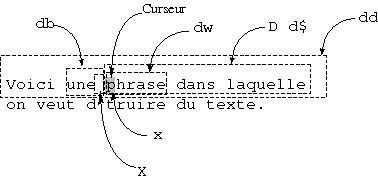
\includegraphics{ann-edt-vi/delete-cmds}
\caption{\label{ann-edt-vi-delfig}Commandes de suppression de texte avec
"{\tt vi}".}
\end{figure}

%%%%%%%%%%%%%%%%%%%%%%%%%%
\subsection{\label{ann-edt-vi-search}Recherche}

%%%%%%%%%%%%%%
\subsubsection{\label{ann-edt-vi-searchcmds}Expression de recherches}

\begin{longtable}{p{4cm}@{\hspace{0.5cm}}p{7cm}}
	\multicolumn{2}{r}{{\sl Suite page suivante $\cdots$}}	\\
\endfoot
\endlastfoot
	\verb*=:set magic=		&
		Autorise les expressions de recherche en utilisant les expressions
		r{\'e}guli{\`e}res (cf. chapitre \ref{reg-exp}). Cette option est positionn{\'e}e
		par d{\'e}faut (cf. section \ref{ann-edt-vi-config}).
		\\[2ex]
	\verb*=:set nomagic=	&
		N'autorise que les symboles "\verb=^=" et "\verb=$=" pour
		les expressions de recherche. Pour plus de pr{\'e}cisions sur les
		options de "{\tt vi}", reportez-vous {\`a} la section \ref{ann-edt-vi-config}.
		\\[2ex]
	\verb=^=				&
		Correspond au d{\'e}but de ligne (idem que les expressions r{\'e}guli{\`e}res,
		cf. \ref{reg-exp}).
		\\[2ex]
	\verb=$=				&
		Correspond {\`a} la fin de ligne (idem que les expressions r{\'e}guli{\`e}res,
		cf. \ref{reg-exp}).
		\\[2ex]
	\verb=.=				&
		Correspond {\`a} n'importe quel caract{\`e}re (idem que les expressions r{\'e}guli{\`e}res,
		cf. \ref{reg-exp}).
		\\[2ex]
	\verb=\<=				&
		Correspond {\`a} un d{\'e}but de mot.
		\\[2ex]
	\verb=\>=				&
		Correspond {\`a} une fin de mot.
		\\[2ex]
	\verb=[={\sl str}\verb=]=	&
		Correspond {\`a} un et un seul caract{\`e}re parmi ceux composant
		"{\sl str}" (idem que les expressions r{\'e}guli{\`e}res,
		cf. \ref{reg-exp}).
		\\[2ex]
	\verb=[^={\sl str}\verb=]=	&
		Correspond {\`a} un et un seul caract{\`e}re diff{\'e}rent de ceux
		composant "{\sl str}" (idem que les expressions r{\'e}guli{\`e}res,
		cf. \ref{reg-exp}).
		\\[2ex]
	\verb=[={\sl a-w}\verb=]=	&
		Correspond {\`a} un et un seul caract{\`e}re entre les caract{\`e}res
		"{\sl a}" et "{\sl w}" (idem que les expressions r{\'e}guli{\`e}res,
		cf. \ref{reg-exp}).
		\\[2ex]
	\verb=*=				&
		Sp{\'e}cifie le nombre d'occurence qu'un caract{\`e}re peut appara{\^\i}tre. Dans
		ce cas, le caract{\`e}re sp{\'e}cifi{\'e} peut appara{\^\i}tre un nombre quelconque
		de fois ( $n \in \{0, \cdots, +\infty\}$).
		\\[2ex]
	\verb=\=				&
		Annule l'interpr{\'e}tation du caract{\`e}re suivant.
		\\[2ex]
	\verb=\\=				&
		Permet de sp{\'e}cifier le caract{\`e}re "\verb=\=". En effet,
		"\verb=\\=" implique que~:
			\begin{itemize}
				\item	le premier "\verb=\=" annule l'{\'e}valuation
						du caract{\`e}re suivant.
				\item	le second caract{\`e}re "\verb=\=" doit {\^e}tre pris
						tel quel.
			\end{itemize}
		\\[2ex]
\end{longtable}

\begin{remarque}
Ce tableau montre que les r{\`e}gles de syntaxes des expressions r{\'e}guli{\`e}res
sont largement utilis{\'e}es dans "{\tt vi}". Tout comme les commandes
"{\tt sed}" et "{\tt awk}" (cf. chapitres \ref{adv-fltrs-sed} et
\ref{adv-fltrs-awk}), "{\tt vi}" fait partie des nombreuses commandes
{\Unix} utilisant la notion des expressions r{\'e}guli{\`e}res.
\end{remarque}

%%%%%%%%%%%%%%
\subsubsection{\label{ann-edt-vi-searchop}Op{\'e}rations de recherche}

\begin{longtable}{p{4cm}@{\hspace{0.5cm}}p{7cm}}
	\multicolumn{2}{r}{{\sl Suite page suivante $\cdots$}}	\\
\endfoot
\endlastfoot
	\verb=%=						&
		Permet de localiser la parenth{\`e}se fermante ou ouvrante correspondant
		{\`a} celle sur laquelle est positionn{\'e} le curseur. Cette fonctionnalit{\'e}
		est op{\'e}rationnelle pour "\verb=(=,\verb=)=", "\verb=[=,\verb=]="
		et "\verb={=,\verb=}=".
		\\[2ex]
	{\tt f}{\sl caract}				&
		Recherche, dans la ligne courrante, le premier caract{\`e}re
		"{\sl caract}", {\bf suivant} la position courrante du curseur.
		\\[2ex]
	{\tt F}{\sl caract}				&
		Recherche, dans la ligne courrante, le premier caract{\`e}re
		"{\sl caract}", {\bf pr{\'e}c{\'e}dant} la position courrante du curseur.
		\\[2ex]
	{\tt t}{\sl caract}				&
		Recherche, dans la ligne courrante, le premier caract{\`e}re
		imm{\'e}diatement pr{\'e}c{\'e}dent {\`a} "{\sl caract}", {\bf suivant} la
		position courrante du curseur.
		\\[2ex]
	{\tt T}{\sl caract}				&
		Recherche, dans la ligne courrante, le premier caract{\`e}re
		imm{\'e}diatement suivant {\`a} "{\sl caract}", {\bf pr{\'e}c{\'e}dant} la
		position courrante du curseur.
		\\[2ex]
	{\tt /}{\sl str}{\returnkey}	&
		Recherche la chaine "{\sl str}" de la position courrante
		du curseur vers la {\bf fin} du fichier.
		\\[2ex]
	{\tt ?}{\sl str}{\returnkey}	&
		Recherche la chaine "{\sl str}" de la position courrante
		du curseur vers le {\bf d{\'e}but} du fichier.
		\\[2ex]
	\verb*=:set ic=					&
		Ignore la diff{\'e}rence entre les majuscules et les minuscules.
		Pour plus d'informations sur les options de "{\tt vi}",
		reportez-vous {\`a} la section \ref{ann-edt-vi-config}.
		\\[2ex]
	\verb*=:set noic=				&
		Fait la diff{\'e}rence entre les majuscules et les minuscules.
		C'est le comportement par d{\'e}faut. Pour plus d'informations
		sur les options de "{\tt vi}", reportez-vous {\`a} la section
		\ref{ann-edt-vi-config}.
		\\[2ex]
\end{longtable}

%%%%%%%%%%%%%%
\subsubsection{\label{ann-edt-vi-searchglob}Recherche globale et substitution}

\begin{longtable}{p{3.5cm}@{\hspace{0.5cm}}p{7.5cm}}
	\multicolumn{2}{r}{{\sl Suite page suivante $\cdots$}}	\\
\endfoot
\endlastfoot
	{\tt :{\sl n,m}s/{\sl str$_1$}/{\sl str$_2$}/{\sl opt}}		&
		Substitue l'expression "{\sl str$_1$}" par "{\sl str$_2$}"
		dans l'espace de travail d{\'e}limit{\'e} par "{\sl n}" et
		"{\sl m}", c'est-{\`a}-dire sur toutes les lignes du fichier
		caract{\'e}ris{\'e}es par "{\sl n}" et "{\sl m}". Les options
		disponibles sont~:
		\begin{description}
			\item[{\rm "{\tt g}"~:}]
				La substitution est globale, c'est-{\`a}-dire qu'elle se
				r{\'e}p{\`e}te autant de fois que n{\'e}cessaire sur chaque ligne
				s{\'e}lectionn{\'e}e. Par d{\'e}faut, la substitution ne s'effectue
				qu'{\bf une seule fois} par ligne.
			\item[{\rm "{\tt c}"~:}]
				Une confirmation est demand{\'e}e avant d'{\'e}ffectuer toute op{\'e}ration
				de substitution. Il suffit d'appuyer sur \key{y} pour
				confirmer et sur {\returnkey} ou \key{n} pour infirmer.
			\item[{\rm "{\tt p}"~:}]
				Les lignes modifi{\'e}es sont affich{\'e}es.
		\end{description}
		Cette commande est identique {\`a} la commande "{\tt s}" de
		"{\tt sed}" (cf. \ref{sed-cmds}).
		\\[2ex]
	\verb*=&=		&
		R{\'e}p{\`e}te l'appel {\`a} la derni{\`e}re commande de substitution "{\tt :s}".
		\\[2ex]
	{\tt :g/{\sl str}/{\sl cmd}}		&
		Ex{\'e}cute la commande "{\sl cmd}" sur toutes les lignes contenant
		l'expression "{\tt str}".
		\\[2ex]
	{\tt :g/{\sl str$_1$}/s/{\sl str$_2$}/{\sl str$_3$/}}	&
		Localise la ligne contenant l'expression "{\sl str$_1$}" et
		y substitue "{\sl str$_2$}" par "{\sl str$_3$/}".
		\\[2ex]
	{\tt :v/{\sl str}/{\sl cmd}}	&
		Ex{\'e}cute la commande "{\sl cmd}" sur toutes les lignes {\bf ne
		contenant pas} l'expression "{\sl str}".
		\\[2ex]
\end{longtable}

%%%%%%%%%%%%%%%%%%%%%%%%%%
\subsection{\label{ann-edt-vi-indent}Indentation de texte}

\begin{longtable}{p{4cm}@{\hspace{0.5cm}}p{7cm}}
	\multicolumn{2}{r}{{\sl Suite page suivante $\cdots$}}	\\
\endfoot
\endlastfoot
	\control{i} ou {\tabkey}									&
		En mode "{\sl insertion}", ins{\`e}re un caract{\`e}re de tabulation
		servant {\`a} l'indentation du programme.
		\\[2ex]
	\verb*,:set ai,												&
		Active ou d{\'e}asctive l'indentation automatique (cf. section
		\ref{ann-edt-vi-config}). Si l'indentation automatique est
		activ{\'e}e, lorsque vous tapez un retour chariot, "{\tt vi}"
		ins{\`e}re automatiquement le nombre n{\'e}cessaire de tabulations afin
		que la nouvelle ligne commence au m{\^e}me niveau que la ligne pr{\'e}c{\'e}dente.
		\\[2ex]
	\verb*,:set sw=,{\sl n}										&
		Fixe, {\bf pour l'affichage}, la taille d'une tabulation. {\bf Attention},
		cette commande ne modifie pas le contenu du fichier en rempla\c{c}ant
		les tabulations par un certain nombre d'espaces, les caract{\`e}res
		de tabulation (code {\ASCII} 9) sont bien pr{\'e}sents dans le fichier.
		"{\tt vi}" interpr{\`e}tera ces caract{\`e}res pour les faire
		correspondre {\`a} une certaine taille, c'est-{\`a}-dire {\`a} un certain nombre
		de colonnes. Par cons{\'e}quent, si vous modifiez la taille des tabulations
		(par d{\'e}faut toutes les 8 colonnes), d'autres {\'e}diteurs pourront
		donner un pr{\'e}sentation diff{\'e}rent de votre code source, {\`a} moins
		biens{\^u}r d'y modifier aussi la taille des taille des tabulations.
		\\[2ex]
	{\sl n}\verb=<<= ou {\sl n}\verb=>>=							&
		D{\'e}cale vers la gauche ("\verb=<<=") ou vers la droite
		("\verb=>>=") les <<{\sl n}" lignes. Si "{\sl n}"
		n'est pas pr{\'e}cis{\'e}, "{\tt vi}" d{\'e}cale la ligne courrante.
		\\[2ex]
	\verb=<={\sl cmd$_{curseur}$} ou \verb=>={\sl cmd$_{curseur}$}	&
		Permet de d{\'e}caler plusieurs lignes vers la gauche ("\verb=<=")
		ou vers la droite ("\verb=>=") en fonction de la commande de
		d{\'e}placement du curseur "{\sl cmd$_{curseur}$}" (cf. section
		\ref{ann-edt-vi-move}).
		\\[2ex]
\end{longtable}

%%%%%%%%%%%%%%%%%%%%%%%%%%
\subsection{\label{ann-edt-vi-cutpaste}Copier/Coller}

"{\tt vi}" dispose d'un certain nombre de {\sl buffer} permettant
de copier ou coller un certain nombre de lignes, de mots ou de caract{\`e}res
qu'il sera possible de replacer n'importe o{\`u} dans le fichier.Ces
{\sl buffers} sont nomm{\'e}s par une lettre allant de "{\tt a}" {\`a}
"{\tt z}".

Dans toute la suite, nous d{\'e}signerons l'op{\'e}ration "{\sl couper}"
par le fait de copier du texte dans un {\sl buffer} et de les
effacer du fichier. De m{\^e}me, nous d{\'e}signerons l'op{\'e}ration "{\sl coller}"
par le fait de placer {\`a} la position courrante du curseur, le contenu
d'un {\sl buffer}.

Dans le tableau suivant, nous d{\'e}signerons l'un de ces {\sl buffers}
par "{\sl (a-z)}".

\begin{longtable}{p{2.5cm}@{\hspace{0.5cm}}p{8.5cm}}
	\multicolumn{2}{r}{{\sl Suite page suivante $\cdots$}}	\\
\endfoot
\endlastfoot
	{\sl n}{\tt yy} ou {\sl n}{\tt Y}	&
		Copie les "{\sl n}" lignes {\`a} partir de la position
		courrante dans le {\sl buffer} par d{\'e}faut. Si "{\sl n}" n'est
		pas pr{\'e}cis{\'e}, alors seule la ligne courrante est m{\'e}moris{\'e}e
		dans le {\sl buffer}.
		\\[2ex]
	{\tt y}{\sl cmd$_{curseur}$}		&
		Copie la partie de texte sp{\'e}cifi{\'e}e par la commande
		de d{\'e}placement de curseur "{\sl cmd$_{curseur}$}" dans
		le {\sl buffer} par d{\'e}faut, {\`a} partir de la position du curseur.
		Par exemple, "{\tt yG}", copie le texte {\`a} partir de la
		position courrante du curseur jusqu'{\`a} la fin de la ligne dans le
		{\sl buffer}.
		\\[2ex]
	{\tt "{\sl (a-z)n}yy}				&
		Copie les "{\sl n}" lignes {\`a} partir de la position
		courrante dans le {\sl buffer} sp{\'e}cifi{\'e}. Si "{\sl n}" n'est pas
		pr{\'e}cis{\'e}, alors seule la ligne courrante est m{\'e}moris{\'e}e
		dans le {\sl buffer}. Par exemple, "{\tt "a10yy}" copie
		les dix lignes suivantes (ligne courrante comprise) dans
		le {\sl buffer} "{\tt a}".
		\\[2ex]
	{\tt "{\sl (a-z)n}dd}				&
		{\sl Coupe} les "{\sl n}" lignes {\`a} partir de la position
		courrante dans le {\sl buffer} sp{\'e}cifi{\'e}. Si "{\sl n}" n'est pas
		pr{\'e}cis{\'e}, alors seule la ligne courrante est m{\'e}moris{\'e}e
		dans le {\sl buffer}. Par exemple, "{\tt "a10dd}" {\sl coupe}
		les dix lignes suivantes (ligne courrante comprise) dans
		le {\sl buffer} "{\tt a}".
		\\[2ex]
	{\tt p} (minuscule)					&
		{\sl Colle} le contenu du {\sl buffer} par d{\'e}faut {\bf apr{\`e}s}�a
		position courrante du curseur. Apr{\`e}s cette op{\'e}ration, le {\sl buffer}
		est vid{\'e}. 
		\\[2ex]
	{\tt P} (majuscule)					&
		{\sl Colle} le contenu du {\sl buffer} par d{\'e}faut {\bf avant}�a
		position courrante du curseur. Apr{\`e}s cette op{\'e}ration, le {\sl buffer}
		est vid{\'e}. 
		\\[2ex]
	{\tt "{\sl (a-z)n}p}�			&
		{\sl Colle} le contenu du {\sl buffer} sp{\'e}cifi{\'e} {\bf apr{\`e}s}�a
		position courrante du curseur. Apr{\`e}s cette op{\'e}ration, le {\sl buffer}
		est vid{\'e}. 
		\\[2ex]
	{\tt "{\sl (a-z)n}P}				&
		{\sl Colle} le contenu du {\sl buffer} sp{\'e}cifi{\'e} {\bf avant}�a
		position courrante du curseur. Apr{\`e}s cette op{\'e}ration, le {\sl buffer}
		est vid{\'e}. 
		\\[2ex]
\end{longtable}

%%%%%%%%%%%%%%%%%%%%%%%%%%
\subsection{\label{ann-edt-vi-mod}Modifier du texte}

\begin{longtable}{p{4cm}@{\hspace{0.5cm}}p{7cm}}
	\multicolumn{2}{r}{{\sl Suite page suivante $\cdots$}}	\\
\endfoot
\endlastfoot
	{\tt r{\sl caract}}						&
		Substitue le caract{\`e}re courrant par le caract{\`e}re "{\sl caract}".
		\\[2ex]
	{\tt R{\sl texte}{\esckey}}				&
		R{\'e}{\'e}crit le texte saisi "{\sl texte}" par dessus ce qui est
		d{\'e}j{\`a} pr{\'e}sent. Ceci {\'e}quivaut au mode "{\sl surimpression}"
		des {\'e}diteurs pleine-page classiques comme "{\tt EVE}" ou
		"{\tt LSEDIT}" sous {\OpenVMS}. Le remplacement de texte
		se termine par la touche {\esckey}. En mode "{\sl insertion}",
		le texte saisi est ins{\'e}r{\'e} {\`a} la position courrante du curseur.
		En mode "{\sl surimpression}", tout ce qui est saisi vient
		s'{\'e}crire par dessus le texte d{\'e}j{\`a} existant.
		\\[2ex]
	{\tt s{\sl texte}{\esckey}}				&
		Substitue le caract{\`e}re courrant avec le texte saisi "{\sl texte}".
		L'insertion du nouveau texte se termine par {\esckey}. Par cons{\'e}quent,
		apr{\`e}s la saisie de la commande "{\tt s}", "{\tt vi}" passe
		en mode "{\sl insertion}".
		\\[2ex]
	{\tt S{\sl texte}{\esckey}} ou {\tt cc{\sl texte}{\esckey}}	&
		Efface la ligne courrante et la substitue par le texte saisi
		"{\sl texte}". L'insertion du nouveau texte se termine par
		{\esckey}. Par cons{\'e}quent, apr{\`e}s la saisie de la commande
		"{\tt s}" ou "{\tt cc}", "{\tt vi}" passe
		en mode "{\sl insertion}".
		\\[2ex]
	{\tt cw{\sl texte}{\esckey}}			&
		Change le mot courrant par le texte saisi "{\sl texte}".
		L'insertion du nouveau texte se termine par {\esckey}. Par cons{\'e}quent,
		apr{\`e}s la saisie de la commande "{\tt cw}", "{\tt vi}" passe
		en mode "{\sl insertion}".
		\\[2ex]
	{\tt C{\sl texte}{\esckey}}				&
		Change le reste de la ligne {\`a} partir de la position courrante par le
		texte saisi "{\sl texte}". L'insertion du nouveau texte se termine
		par {\esckey}. Par cons{\'e}quent, apr{\`e}s la saisie de la commande
		"{\tt C}", "{\tt vi}" passe en mode "{\sl insertion}".
		\\[2ex]
	{\tt c{\sl curs$_{cmd}$texte}{\esckey}}	&
		De fa\c{c}on plus g{\'e}n{\'e}rale, la commande "{\tt c}" suivie d'une
		commande "{\tt vi}" de d{\'e}placement de curseur (cf. section
		\ref{ann-edt-vi-move}), change le texte correspondant avec ce qui a
		{\'e}t{\'e} saisi, jusqu'{\`a} ce que la touche {\esckey} soit press{\'e}e.
		Par cons{\'e}quent, apr{\`e}s la saisie de la commande
		"{\tt c{\sl curs$_{cmd}$}}", "{\tt vi}" passe en mode
		"{\sl insertion}".
		\\[2ex]	
	{\tt J}									&
		Rassemble la ligne courrante et la ligne suivante sur une seule et
		m{\^e}me ligne.
		\\[2ex]
	{\tt {\sl n}J}							&
		Rassemble les "{\sl n}" lignes, y compris la ligne courrante, sur
		une seule et m{\^e}me ligne.
		\\[2ex]
\end{longtable}

%%%%%%%%%%%%%%%%%%%%%%%%%%
\subsection{\label{ann-edt-vi-place}Placement direct du curseur et ajustement
			du texte {\`a} l'{\'e}cran}

\begin{longtable}{p{4cm}@{\hspace{0.5cm}}p{7cm}}
	\multicolumn{2}{r}{{\sl Suite page suivante $\cdots$}}	\\
\endfoot
\endlastfoot
	{\tt H}									&
		Ram{\`e}ne le curseur sur la premi{\`e}re ligne de l'{\'e}cran, ligne qui n'est
		pas forc{\'e}ment la premi{\`e}re ligne du fichier.
		\\[2ex]
	{\tt {\sl n}H}							&
		Ram{\`e}ne le curseur sur la $n^{e}$ ligne de l'{\'e}cran, ligne qui n'est pas
		forc{\'e}ment la $n^{e}$ ligne du fichier.
		\\[2ex]
	{\tt M}									&
		Am{\`e}ne le curseur au milieu de l'{\'e}cran.
		\\[2ex]
	{\tt L}									&
		Am{\`e}ne le curseur sur la derni{\`e}re ligne de l'{\'e}cran, ligne qui n'est pas
		forc{\'e}ment la derni{\`e}re ligne du fichier.
		\\[2ex]
	{\tt {\sl n}L}							&
		Am{\`e}ne le curseur sur la $n^{e}$ ligne de l'{\'e}cran en partant du bas de
		l'{\'e}cran.
		\\[2ex]
	\control{e}								&
		D{\'e}cale l'affichage d'une ligne vers le haut.
		\\[2ex]
	\control{y}								&
		D{\'e}cale l'affichage d'une ligne vers le bas.
		\\[2ex]
	\control{u}								&
		D{\'e}cale l'affichage d'une demi page vers le haut.
		\\[2ex]
	\control{d}								&
		D{\'e}cale l'affichage d'une demi page vers le bas.
		\\[2ex]
	\control{b}								&
		D{\'e}cale l'affichage d'une demi page vers le haut. Cette fonction est aussi
		disponible avec la touche "{\sl Page Pr{\'e}c{\'e}dente}".
		\\[2ex]
	\control{f}								&
		D{\'e}cale l'affichage d'une page vers le bas. Cette fonction est aussi
		disponible avec la touche "{\sl Page Suivante}".
		\\[2ex]
	\control{l} (lettre "{\tt l}")		&
		Rafra{\^\i}chit l'{\'e}cran. Cette fonction {\'e}quivaut {\`a} \control{w} avec les
		{\'e}diteurs <<{\tt EVE}" ou "{\tt LSEDIT}" sous {\OpenVMS}.
		\\[2ex]
	{\tt z{\returnkey}}						&
		D{\'e}cale l'affichage de telle sorte que la ligne courrant devienne la
		premi{\`e}re ligne affich{\'e}e en haut de l'{\'e}cran.
		\\[2ex]
	{\tt {\sl n}z{\returnkey}}				&
		D{\'e}cale l'affichage de telle sorte que la $n^{e}$ ligne affich{\'e}e en partant
		du haut, devienne la premi{\`e}re ligne affich{\'e}e {\`a} l'{\'e}cran.
		\\[2ex]
	{\tt z.}								&
		D{\'e}cale l'affiche de telle sorte que la ligne courrante devienne celle
		du milieu de l'{\'e}cran.
		\\[2ex]
	{\tt {\sl n}z.}							&
		D{\'e}cale l'affichage de telle sorte que la $n^{e}$ ligne affich{\'e}e en partant
		du haut, devienne celle du milieur de l'{\'e}cran.
		\\[2ex]
	{\tt z-}								&
		D{\'e}cale l'affichage de telle sorte que la ligne courrante devienne
		la derni{\`e}re ligne affich{\'e}e en bas de l'{\'e}cran.
		\\[2ex]
	{\tt {\sl n}z-}							&
		D{\'e}cale l'affichage de telle sorte que la $n^{e}$ ligne affich{\'e}e en partant
		du haut, devienne la derni{\`e}re ligne affich{\'e}e en bas de l'{\'e}cran.
		\\[2ex]
\end{longtable}

\begin{remarque}
L'ensemble de ces commandes s'adaptent en fonction de la taille de l'{\'e}cran,
c'est-{\`a}-dire du nombre de lignes et de colonnes.
\end{remarque}


%%%%%%%%%%%%%%%%%%%%%%%%%%
\subsection{\label{ann-edt-vi-sh}Interaction avec le {\sl shell}}

\begin{longtable}{p{4cm}@{\hspace{0.5cm}}p{7cm}}
	\multicolumn{2}{r}{{\sl Suite page suivante $\cdots$}}	\\
\endfoot
\endlastfoot
	\verb*=:!={\sl commande}					&
		Ex{\'e}cute la commande dans un sous processus. Cette commande peut
		{\^e}tre n'importe quelle commande {\sl shell}, y compris un appel
		{\`a} une autre session "{\tt vi}". Lors de la saisie de la commande
		au niveau du {\sl prompt} de "{\tt vi}", il est possible
		d'utiliser les caract{\`e}res sp{\'e}ciaux suivants~:
		\\[2ex]
		&
		\begin{tabular}{l@{\hspace{1ex}}p{5cm}}
			\verb=%=	& correspond au nom du fichier en train d'{\^e}tre
				{\'e}dit{\'e}.\\
			\verb=#=	& correspond au nom du dernier fichier {\'e}dit{\'e}.\\
		\end{tabular}
		\\[2ex]
		&
		L'interpr{\'e}teur de commandes utilis{\'e} par d{\'e}faut est le Bourne Shell
		("\verb=/bin/sh=". Cette valeur peut {\^e}tre modifi{\'e}e gr{\^a}ce {\`a}
		la commande "\verb*,:set shell=,{\sl chemin}" (cf.
		\ref{ann-edt-vi-config}).
		\\[2ex]
	\verb*=:!!=									&
		R{\'e}ex{\'e}cute la derni{\`e}re commande {\sl shell}, c'est-{\`a}-dire la
		derni{\`e}re commande "\verb*=:!={\sl commande}".
		\\[2ex]
	\verb*=:r! ={\sl commande}					&
		Inclut dans le fichier {\`a} la position courrante du curseur
		la sortie standard de la commande "{\sl commande}".
		\\[2ex]
	\verb*=:f ={\sl nouv\_fichier}				&
		Renomme le fichier courrant sous le nouveau nom
		"{\sl nouv\_fichier}". Dans ce cas de figure, le fichier
		{\'e}dit{\'e} change de nom sur le disque mais aussi pour "{\tt vi}".
		Ainsi, toute op{\'e}ration future de sauvegarde se fera sous le
		nouveau nom de fichier.
		\\[2ex]
	\verb*=:w !={\sl commande}					&
		Sauvegarde le fichier courrante et envoie son contenu sur l'entr{\'e}e
		standard de la commande "{\sl commande}".
		\\[2ex]
	\verb*=:cd ={\sl r{\'e}pertoire}			&
		Change le r{\'e}pertoire par d{\'e}faut de "{\tt vi}". Si aucun r{\'e}pertoire
		n'est sp{\'e}cifi{\'e}, le contenu de la variable d'environnement
		"{\tt HOME}" est utilis{\'e}.
		\\[2ex]
	\verb*=:sh=									&
		D{\'e}marre un sous processus de "{\tt vi}" dans lequel sera
		ex{\'e}cut{\'e} un nouvel interpr{\'e}teur de commandes. Pour revenir {\`a}
		"{\tt vi}", il suffit de taper la commande "{\tt exit}"
		ou \control{d}, commande ou s{\'e}quence de touche permettant
		de terminer une session {\sl shell} (cf. \ref{bcpts-login}
		et \ref{test-loop-break}).
		\\[2ex]
	\verb*=:so ={\sl fichier}						&
		Lit et ex{\'e}cute les commandes {\sl shell} pr{\'e}sentes dans le
		fichier "{\sl fichier}".
		\\[2ex]
	\verb*=!={\sl cmd$_{curseur}$\verb*= =commande}	&
		Envoie le texte s{\'e}lectionn{\'e} par la commande de d{\'e}placement
		de curseur "{\sl cmd$_{curseur}$}" {\`a} la commande {\sl shell}
		"{\sl commande}". Le texte correspondant {\`a} la commande
		de d{\'e}placement du curseur est remplac{\'e} par la sortie standard
		de la commande. Par exemple~:
		\\[2ex]
		&
		\begin{tabular}{l@{\hspace{1ex}}p{5cm}}
			\verb*=!w ls -l={\returnkey} 	&
			envoie le mot situ{\'e} au niveau du curseur {\`a} la commande
			"{\tt ls -l}". Le mot en question est remplac{\'e} par
			le r{\'e}sultat de la commande.
			\\[2ex]
			\verb*=!}sort={\returnkey}		&
			S{\'e}lectionne le texte de la position courrante du curseur
			jusqu'{\`a} la fin du paragraphe et le trie gr{\^a}ce {\`a} la commande
			"{\tt sort}". Le texte s{\'e}lectionn{\'e} est remplac{\'e} par le
			r{\'e}sultat du tri.
		\end{tabular}
		\\[2ex]
\end{longtable}

%%%%%%%%%%%%%%%%%%%%%%%%%%
\subsection{\label{ann-edt-vi-macros}Macros et abr{\'e}viations}

\begin{longtable}{p{4cm}@{\hspace{0.5cm}}p{7cm}}
	\multicolumn{2}{r}{{\sl Suite page suivante $\cdots$}}	\\
\endfoot
\endlastfoot
	\verb*=:map ={\sl touche}\verb*= ={\sl s{\'e}quence$_{cmds}$}	&
		Associe la s{\'e}quence de commandes
		"{\sl s{\'e}quence$_{cmds}$}" {\`a} la touche "{\sl touche}".
		Ainsi, d{\`e}s que cette touche est appuy{\'e}e, la s{\'e}quence de commandes
		est ex{\'e}cut{\'e}e.
		\\[2ex]
	\verb*=:map=													&
		Affiche l'ensemble des d{\'e}finitions effectu{\'e}es, c'est-{\`a}-dire
		l'ensemble des "{\sl macros}" de "{\tt vi}" cr{\'e}{\'e}es
		gr{\^a}ce {\`a} la commande pr{\'e}c{\'e}dente.
		\\[2ex]
	\verb*=:unmap ={\sl touche}										&
		D{\'e}truit l'association entre une touche et la s{\'e}quence de
		commandes pr{\'e}c{\'e}demment faite. Cette commande d{\'e}truit donc
		la macro associ{\'e}e {\`a} la touche "{\sl touche}".
		\\[2ex]
	\verb*=:ab ={\sl chaine$_1$}\verb*= ={\sl chaine$_2$}			&
		Permet de d{\'e}finir une abr{\'e}viation. Lorsque "{\sl chaine$_1$}"
		est saisi, "{\tt vi}" la substitue par "{\sl chaine$_2$}".
		\\[2ex]
	\verb*=:ab=														&
		Affiche l'ensemble des abr{\'e}viations d{\'e}finies.
		\\[2ex]
	\verb*=:una ={\sl chaine}										&
		D{\'e}truit l'abr{\'e}viation "{\sl chaine}".
		\\[2ex]
\end{longtable}

La commande "{\tt :map}" permer de d{\'e}finir des s{\'e}quences de commandes
ou "{\sl macros}" "{\tt vi}". En effet, par d{\'e}finition, une
macro, comme en langage C ou n'importe quel logiciel, est une s{\'e}rie de
commandes ou d'actions de base regroup{\'e}es sous un nom et appelable
par l'utilisateur.

Si l'option "{\tt timeout}" est positionn{\'e}e (cf. section
\ref{ann-edt-vi-config}), toute ex{\'e}cution de macros ne peut d{\'e}passer une
seconde. Par cons{\'e}quent, si vous utilisez des macros importantes,
d{\'e}sactivez cette option.

Sachant que les commandes "{\tt vi}" utilisent des caract{\`e}res de
contr{\^o}le en mode commande, il est possible de les ins{\'e}rer dans la
d{\'e}finition des macros gr{\^a}ce {\`a} la s{\'e}quence \control{v} (cf. section
\ref{ann-edt-vi-insert}). De m{\^e}me, le caract{\`e}re "{\tt "}" est utilis{\'e}
dans les commandes "{\tt vi}" (cf. sections \ref{ann-edt-vi-undo}
et \ref{ann-edt-vi-cutpaste}). Par cons{\'e}quent, s'il doit {\^e}tre utilis{\'e}
dans une macro dans un autre cadre que celui d'une commande le r{\'e}f{\'e}ren\c{c}ant,
il doit {\^e}tre pr{\'e}c{\'e}d{\'e} du caract{\`e}re "\verb=\=".

\begin{remarque}
Les touches inutilis{\'e}es sous "{\tt vi}" sont~:
\begin{itemize}
	\item	les touches de fonction,
	\item	les touches "{\tt K}", "{\tt V}", "{\tt g}",
			"{\tt q}", "{\tt v}", "\verb=*=" et "{\tt =}". 
\end{itemize}
\end{remarque}

\begin{example}
\verb*=:map v /Je =\control{v}{\esckey}\verb*=dwiTu =\control{v}{\esckey}{\esckey}
\\[2ex]
Lorsque la touche \key{v} est appuy{\'e}e {\bf en mode "{\sl commande}"},
les actions suivantes sont ex{\'e}cut{\'e}es~:
\begin{enumerate}
	\item	Recherche de la chaine "\verb*=Je ="
			("\verb*=/Je ={\esckey}"),
	\item	Efface le mot courrant ("\verb=dw="),
	\item	Ins{\`e}re la chaine "\verb*=Tu ={\esckey}"
			("\verb*=iTu =\control{v}{\esckey}"),
	\item	Termine le mode "{\sl insertion}" ("{\esckey}").
\end{enumerate}
\end{example}

Dans la section \ref{ann-edt-vi-config}, vous trouverez un ensemble
d'abr{\'e}viations d{\'e}finies par d{\'e}faut dans "{\tt vi}". La commande
"\verb*=:ab ={\sl chaine$_1$}\verb*= ={\sl chaine$_2$}" permet
de d{\'e}finir celles qui vous seront propres.

%%%%%%%%%%%%%%%%%%%%%%%%%%
\subsection{\label{ann-edt-vi-config}Commandes de configuration de "{\tt vi}"}

"{\tt vi}" dispose d'un certain nombre d'options permettant de
param{\`e}trer son fonctionnement et l'environnement de travail. Celles-ci
sont regroup{\'e}es en trois cat{\'e}gories~:
\begin{description}
	\item[{\rm les options de type "{\sl bascule}"~:}]\mbox{}\\
		Dans ce cas de figure, l'option correspond {\`a} deux
		{\'e}tat possible~:
		\begin{itemize}
			\item	activ{\'e},
			\item	d{\'e}sactiv{\'e}.
		\end{itemize}
	\item[{\rm les options de type "{\sl num{\'e}rique}"~:}]\mbox{}\\
		{\`A} ces options sont associ{\'e}es des valeurs num{\'e}riques.
	\item[{\rm les options de type "{\sl chaine}"~:}]\mbox{}\\
		Comme pour le type pr{\'e}c{\'e}dent, l'option est associ{\'e}e {\`a} une valeur
		de type "{\sl chaine de caract{\`e}res}".
\end{description}

\begin{longtable}{p{4cm}@{\hspace{0.5cm}}p{7cm}}
	\multicolumn{2}{r}{{\sl Suite page suivante $\cdots$}}	\\
\endfoot
\endlastfoot
	\verb*=:set=								&
		Affiche toutes les options {\bf qui ont {\'e}t{\'e} modifi{\'e}es par rapport
		{\`a} la configuration par d{\'e}faut}, et la valeur ou l'{\'e}tat associ{\'e}.
		\\[2ex]
	\verb*=:set all=							&
		Affiche toutes les options et la valeur ou l'{\'e}tat associ{\'e}.
		\\[2ex]
	\verb*=:set ={\sl option}					&
		Si l'option est de type "{\sl bascule}", elle
		est arm{\'e}e. Si elle est d'un autre type ("{\sl chaine}" ou
		"{\sl num{\'e}rique}", la valeur associ{\'e}e est affich{\'e}e.
		\\[2ex]
	\verb*=:set no={\sl option}					&
		Ce cas de figure n'est valable que si l'option est de type
		"{\sl bascule}". Dans ce cas, elle est d{\'e}sactiv{\'e}e.
		\\[2ex]
	\verb*=:set inv={\sl option}				&
		Inverse l'{\'e}tat d'une option de type <<n {\sl bascule}".
		\\[2ex]
	\verb*=:set ={\tt {\sl option}={\sl value}}	&
		Fixe la valeur associ{\'e}e {\`a} une option de type "{\sl chaine}" ou
		"{\sl num{\'e}rique}".
		\\[2ex]
	\verb*=:set ={\tt {\sl option}?}			&
		Affiche la valeur ou l'{\'e}tat associ{\'e}e {\`a} l'option sp{\'e}cifi{\'e}e.
		\\[2ex]
\end{longtable}

\begin{longtable}{|l|c|c|l|p{6cm}|}
	\hline
		\multicolumn{5}{|r|}{Suite de la page pr{\'e}c{\'e}dente $\cdots$}	\\
	\hline
		\multicolumn{1}{|c|}{Option}			&
		\multicolumn{1}{|c|}{Abbr{\'e}viation}	&
		\multicolumn{1}{|c|}{Type}				&
		\multicolumn{1}{|c|}{D{\'e}faut}		&
		\multicolumn{1}{|c|}{Description}		\\
	\hline
\endhead
	\hline
		\multicolumn{1}{|c|}{Option}			&
		\multicolumn{1}{|c|}{Abbr{\'e}viation}	&
		\multicolumn{1}{|c|}{Type}				&
		\multicolumn{1}{|c|}{D{\'e}faut}		&
		\multicolumn{1}{|c|}{Description}		\\
	\hline
\endfirsthead
	\hline
		\multicolumn{5}{|r|}{Suite page suivante $\cdots$}	\\
	\hline
\endfoot
	\hline
\endlastfoot
	{\tt autoindent}	&	{\tt ai}	&	bascule	&	non				&
		Lorsque cette option est activ{\'e}e, les tabulations sont automatiquement ins{\'e}r{\'e}es en
		mode "{\sl insertion}" afin que les lignes soient align{\'e}es sur une m{\^e}me colonne.
		Pour revenir en arri{\`e}re, au niveau de l'alignement des colonnes, il suffit de repasser
		en mode "{\sl commande}" et positionner le curseur {\`a} la colonne souhait{\'e}e.
		\\[2ex]
	{\tt directory}		&	{\tt dir}	&	chaine	&	{\tt /tmp}		&
	    Sp{\'e}cifie le r{\'e}pertoire temporaire de "{\tt vi}" pour stocker ses informations.
	    Ce r{\'e}pertoire contiendra, entre autre, un fichier que vous pourrez utiliser en
	    cas d'interruption de la session "{\tt vi}" et retrouver toutes les modifications
	    que vous aurez effectu{\'e}es (cf. option "{\tt -v}" {\`a} la section \ref{ann-edt-vi-start}).
		\\[2ex]
	{\tt errorbells}	&	{\tt eb}	&	bascule	&	non				&
		Pr{\'e}c{\`e}de tous les messages d'erreur par un "{\sl bip}".
		\\[2ex]
	{\tt ignorecase}	&	{\tt ic}	&	bascule	&	non				&
		Ignire les majuscules/minuscules lors des op{\'e}rations de recherche.
		\\[2ex]
	{\tt insertmode}	&	{\tt im}	&	bascule	&	non				&
		D{\'e}marre la session "{\tt vi}" en mode "{\sl insertion}". Par d{\'e}faut,
		"{\tt vi}" d{\'e}marre en mode "{\sl commande}".
		\\[2ex]
	{\tt lines}			&				&	nombre	&	25				&
		Sp{\'e}cifie le nombre de lignes {\`a} afficher {\`a} l'{\'e}cran. Par d{\'e}faut, le nombre de lignes est
		"25" ou, plus pr{\'e}cis{\'e}ment le nombre de lignes affichable par le terminal.
		Ce param{\`e}trage est accessible par la commande "{\tt stty(1)}" ou "{\tt resize(1)}".
		La premi{\`e}re permet de sp{\'e}cifier les param{\`e}tres du terminal manuellement. La seconde
		interroge le terminal pour obtenir ces caract{\'e}ristiques.
		\\[2ex]
	{\tt list}			&				&	bascule	&	non				&
		Affiche tous les caract{\`e}res invisibles. Lorsque cette option est activ{\'e}e, nous
		aurons, entre-autre~:
		\\
		& & & &
		\begin{tabular}{l@{\hspace{2ex}}p{5cm}}
			\verb=^I=	&	Tabulation		\\
			\verb=$=	&	Fin de ligne	\\
		\end{tabular}
		\\[2ex]
	{\tt magic}			&				&	bascule	&	oui				&
		Autorise les expressions r{\'e}guli{\`e}res pour les op{\'e}rations de recherche.
		\\[2ex]
	{\tt makeprg}		&	{\tt mp}	&	chaine	&	{\tt make}		&
		Sp{\'e}cifie le nom de l'utilitaire permettant de g{\'e}n{\'e}rer les d{\'e}pendances entre les
		diff{\'e}rents fichiers source et les ex{\'e}cutables {\`a} g{\'e}n{\'e}rer. Par d{\'e}faut, la commande
		{\Unix}�tilis{\'e}e est "{\tt make(1)}".
		\\[2ex]
	{\tt number}		&	{\tt nu}	&	bascule	&	non				&
		Affiche le num{\'e}ro de chaque ligne.
		\\[2ex]
	{\tt readonly}		&	{\tt ro}	&	bascule	&	non				&
		Le fichier courrant passe en lecture seule. Il est possible de l'{\'e}diter, mais
		la sauvegarde n'est pas accessible. Cependant, si les droits d'acc{\`e}s au fichier
		le permettent, la commande "\verb=:w!=" force la sauvegarde (cf. section
		\ref{ann-edt-vi-quit}). Ce mode est positionn{\'e} par d{\'e}faut si les droits d'acc{\`e}s
		au fichier n'autorisent que la lecture.
		\\[2ex]
	{\tt remap}			&				&	bascule	&	oui				&
		Autorise l'appel de macros {\`a} l'int{\'e}rieurs de macros ({\sl macros} r{\'e}cursives).
		\\[2ex]
	{\tt report}		&				&	nombre	&	2				&
		Sp{\'e}cifie le nombre de lignes minimales pour que "{\tt vi}" puisse afficher
		ses informations.
		\\[2ex]
	{\tt revins}		&	{\tt ri}	&	bascule	&	non				&
		Au lieu d'ins{\'e}rer du texte de la gauche vers la droite (sens normal pour l'alphabet romain)
		mais de la droite vers la gauche.
		\\[2ex]
	{\tt ruler}			&	{\tt ru}	&	bascule	&	non				&
		Affiche la position courrante du curseur (ligne$\times$colonne) dans la zone
		o{\`u} "{\tt vi}" inscrit ses informations.
		\\[2ex]
	{\tt scroll}		&				&	nombre	&	12				&
		Pr{\'e}cise le nombre de lignes {\`a} prendre en compte pour les commandes
		\control{u}, \control{d}, \control{b} et \control{f}
		(cf. section \ref{ann-edt-vi-place}).
		\\[2ex]
	{\tt scrolljump}	&	{\tt sj}	&	nombre	&	1				&
		Pr{\'e}cise le nombre de lignes minimal pour les passages aux
		{\'e}crans pr{\'e}c{\'e}dents et suivants.
		\\[2ex]
	{\tt shell}			&	{\tt sh}	&	chaine	&	{\tt sh}		&
		Pr{\'e}cise l'interpr{\'e}teur de commande {\`a} utiliser par d{\'e}faut
		pour les inter-actions avec le "{\sl shell}"
		(cf. section \ref{ann-edt-vi-sh}).
		\\[2ex]
	{\tt shiftwidth}	&	{\tt sw}	&	nombre	&	8				&
		Pr{\'e}cise la taille des d{\'e}calages pour les commandes
		"\verb=<=" et "\verb=>=" (cf. section
		\ref{ann-edt-vi-indent}).
		\\[2ex]
	{\tt shortname}		&	{\tt sn}	&	bascule	&	non				&
		Assure la compatibilit{\'e} avec des syst{\`e}mes de fichier type
		{\DOS}, c'est-{\`a}-dire des noms de fichiers en majuscules, ne
		comportant que huits caract{\`e}res au maximum avec une extension
		d'au plus trois caract{\`e}res.
		\\[2ex]
	{\tt showmatch}		&	{\tt sm}	&	bascule	&	non				&
		Si cette option est activ{\'e}e, "{\tt vi}" indique {\`a} l'utilisateur
		quelle est la {\sl parenth{\`e}se} ouvrante correspondante d{\`e}s qu'il
		saisit l'un des caract{\`e}res suivants~:
		\begin{itemize}
			\item <<{\tt )}" (caract{\`e}re associ{\'e} "{\tt (}"),
			\item "\verb=}=" (caract{\`e}re associ{\'e} "\verb={="),
			\item "\verb=]=" (caract{\`e}re associ{\'e} "\verb=[="),
		\end{itemize}
		\\[2ex]
	{\tt showmode}		&	{\tt smd}	&	bascule	&	oui				&
		Si cette option est active, "{\tt vi}" indique le mode
		courrant.
		\begin{itemize}
			\item	si le mode courrant est le mode "{\sl insertion}",
					"{\tt vi}" inscrit "{\tt --~INSERT~--}",
			\item	si le mode courrant est le mode "{\sl commande}",
					{\bf aucune information} n'est sp{\'e}cifi{\'e}e dans la ligne
					d'{\'e}tat.
		\end{itemize}
		{\bf Attention}, dans certains cas, cette option n'est pas positionn{\'e}e
		par d{\'e}faut.
		
		De m{\^e}me, pour certaines versions de "{\tt vi}", les informations
		affich{\'e}es sont plus explicites~:
		\begin{itemize}
			\item	"{\tt vi}" inscrit "{\tt --~INSERT~--}" si
					l'utilisateur ins{\`e}re du texte {\bf avant} le curseur
					(commandes \key{i}, \key{I}, \key{O}, etc. --
					cf. section \ref{ann-edt-vi-insert}),
			\item	"{\tt vi}" inscrit "{\tt --~INSERT~--}" si
					l'utilisateur ins{\`e}re du texte {\bf apr{\`e}s} le curseur
					(commandes \key{a}, \key{A}, \key{o}, etc. --
					cf. section \ref{ann-edt-vi-insert}).
		\end{itemize}			
		\\[2ex]
	{\tt sidescroll}	&	{\tt ss}	&	nombre	&	0				&
		Nombre de colonnes minimales pour le {\sl scrolling} horizontal.
		\\[2ex]
	{\tt tabstop}		&	{\tt ts}	&	nombre	&	8				&
		Pr{\'e}cise la taille des tabulations.
		\\[2ex]
	{\tt term}			&				&	chaine	&					&
		Type de terminal sur lequel l'utilisateur travaille. "{\tt vi}"
		prend, par d{\'e}faut, le contenu de la variable d'environnement
		du {\sl shell}~: "{\tt TERM}".
		\\[2ex]
	{\tt terse}			&				&	bascule	&	non				&
		Utilise les messages d'erreurs abr{\'e}g{\'e}s.
		\\[2ex]
	{\tt textauto}		&	{\tt ta}	&	bascule	&	oui				&
		D{\'e}tecte les caract{\`e}res utilis{\'e}s pour s{\'e}parer les lignes d'un fichier.
		"{\tt vi}" positionne alors automatiquement l'option
		"{\tt textmode}". En effet,
		\begin{itemize}
			\item	sous {\DOS}, chaque ligne est s{\'e}par{\'e}e par les deux caract{\`e}res
					{\sl carriage-return}--{\sl line-feed} (respectivement
					{\ASCII}(13) et {\ASCII}(10)),
			\item	sous {\Unix}, chaque ligne n'est s{\'e}par{\'e}e que par le
					caract{\`e}re {\sl line-feed} ({\ASCII}(10)),
			\item	sous {\MacOS}, chaque ligne n'est s{\'e}par{\'e}e que par le
					caract{\`e}re {\sl carriage-return}  ({\ASCII}(13)).
		\end{itemize}
		\\[2ex]
	{\tt textmode}		&	{\tt tx}	&	bascule	&	non				&
		Utilise les caract{\`e}res de fin de ligne de {\DOS}.
		\\[2ex]
	{\tt textwidth}		&	{\tt tw}	&	nombre	&	0				&
		Sp{\'e}cifie la longueur maximale d'une ligne en mode
		"{\sl insertion}".
		\\[2ex]
	{\tt timeout}		&				&	bascule	&	oui				&
		Prend en compte la valeur de la temporisation fix{\'e}e par
		l'option "{\tt timeoutlen}" (ou "{\tt tm}" pour
		l'ex{\'e}cution des macros "{\tt vi}". Ainsi, aucune macros
		ne pourra s'ex{\'e}cuter plus de "{\tt timeoutlen}"
		millisecondes.
		\\[2ex]
	{\tt timeoutlen}	&	{\tt tm}	&	nombre	&	1000			&
		Fixe la valeur de la temporisation pour l'option
		"{\tt timeout}". La valeur est exprim{\'e}e en {\bf millisecondes}.
		\\[2ex]
	{\tt visualbell}	&	{\tt vb}	&	bascule	&	non				&
		Au lieu d'avoir un signal sonore, "{\tt vi}" fait flasher
		l'{\'e}cran.
		\\[2ex]
	{\tt warn}			&				&	bascule	&	oui				&
		Affiche un message si, lors d'une sortie de l'{\'e}diteur,
		le fichier n'a pas {\'e}t{\'e} sauvegard{\'e}. Typiquement
		le message sera "{\tt No write since last change.}".
		\\[2ex]
	{\tt wildchar}		&	{\tt wc}	&	nombre	&	{\tabkey}		&
		Touche ou caract{`e}re utilis{\'e} pour compl{'e}ter
		automatiquement les nom de fichiers. Le nombre sp{\'e}cifi{\'e}
		correspond au code {\ASCII} du caract{`e}re concern{\'e}. Le
		comportement par d{\'e}faut est similaire {\`a} celui
		observable avec "{\tt tcsh}" et "{\tt bash}".
		\\[2ex]
	{\tt wrap}			&				&	bascule	&	oui				&
		Lorsque cette option est active, si la saisie d{\'e}passe
		la largeur maximale de la fen{\^e}tre d'affichage, un retour
		automatique {\`a} la ligne est effectu{\'e} {\bf sans pour
		autant avoir le caract{\`e}re {\returnkey} ins{\'e}r{\'e}
		dans le texte}. Si cette option n'est pas active, l'affichage
		se d{\'e}calera horizontalement.
		\\[2ex]
	{\tt wrapmargin}	&	{\tt wm}	&	nombre	&	0				&
		Le retour {\`a} la ligne suivante s'effectue {\`a} partir de la
		colonne "{\sl nombre de colonnes de la fen{\^e}tre}" -
		"{\sl valeur associ{\'e}e {\`a} l'option {\tt wrapmargin}}".
		Cette op{\'e}ration s'ex{\'e}cute si l'option "{\tt wrap}"
		est active.
		\\[2ex]
\end{longtable}

%%%%%%%%%%%%%%%%%%%%%%%%%%
\subsection{\label{ann-edt-vi-exrc}Fichier d'initialisation de
	"{\tt vi}"~: "{\tt .exrc}"}

L'ensemble des commandes de "{\tt vi}" permettant de d{\'e}finir
son environnement de travail, c'est-{\`a}-dire l'ensemble des
commandes appelable {\`a} partir du {\sl prompt} de l'{\'e}diteur
(caract{\`e}re "{\tt :}") sont m{\'e}morisables dans un fichier
de configuration~: le fichier "{\tt .exrc}" situ{\'e} dans
le r{\'e}pertoire de connexion de l'utilisateur (r{\'e}pertoire
contenu dans la variable d'environnement "{\tt HOME}").

Toutes ces commandes, vues dans les sections pr{\'e}c{\'e}dentes
peuvent y {\^e}tre plac{\'e}e {\bf sans les faire pr{\'e}fixer
du caract{\`e}re "{\tt :}"}.

Par exemple~:
\begin{quote}
\begin{verbatim}
set number
set autoindent
map v d$
\end{verbatim}
\end{quote}
permet, pour toutes les sessions "{\tt vi}" qui seront lanc{\'e}es~:
\begin{itemize}
	\item	d'afficher les num{\'e}ros des lignes,
	\item	de faire de l'indentation automatique,
	\item	de d{\'e}finir la macro "\key{v}".
\end{itemize}

Le nom de ce fichier est param{\`e}trable gr{\^a}ce {\`a} la variable
d'environnement "{\tt EXRC}" qui contiendra le chemin absolu et
le nom du nouveau fichier de configuration.

Par cons{\'e}quent, {\`a} chaque nouvelle session "{\tt vi}",
l'{\'e}diteur suivra le processus suivant~:
\begin{enumerate}
	\item	"{\tt vi}" regarde si la variable d'environnement
			"{\tt EXRC}" est d{\'e}finie. Si oui, il m{\'e}morise
			le nouveau nom du fichier de configuration. Si non,
			il prendra la valeur par d{\'e}faut ("{\tt \$HOME/.exrc}").
	\item	"{\tt vi}" regarde si le fichier de configuration
			existe et est accessible en lecture. Si oui, il charge son
			contenu. Si non, aucune op{\'e}ration n'est effectu{\'e}e.
\end{enumerate}
